\section{Conduction/Diffusion thermique}

    \subsection{Vecteur densité de courant thermique}

        On modélise le caractère directionnel du flux thermique surfacique $\varphi$ par un vecteur densité de courant thermique, voir la Figure~\ref{fig:vecteur_densite_courant_thermique}.

        \begin{figure}
            \centering
            \tikzsetnextfilename{vecteur_densite_courant_thermique}
            \begin{tikzpicture}[scale=1]  
                % \helpgrid{3}{3}
                \draw [thick] (0,0) ellipse (1cm and 1.5cm) node [below, shift=({0,-0.25})] {$\d S$};
                \draw [color=black,smooth, pattern=north west lines] (0,0) circle (0.25);
                \draw [thick, ->] (0,0)--++(2,0) node [above] {$\vec{n}$};
                \draw [-stealth, thick, red!50!black, text=red] (0, 0)--++(1.5,1.2) node [above,pos=0.9] {$\vec{j_{\text{th}}}$};
            \end{tikzpicture}
            \caption{Définition du vecteur densité de courant thermique.}    
            \label{fig:vecteur_densite_courant_thermique}
        \end{figure}

        \begin{definition}[Vecteur densité de courant thermique]
            On définit le \textbf{vecteur densité de courant thermique} par la formule
            \begin{equation}
                \varphi=\vec{j_{\text{th}}}\cdot\vec{n}.
            \end{equation}
            Ainsi, la puissance thermique est
            \begin{equation}
                \boxed{
                    P_{\text{th}}=\iint_{S}\vec{j_{\text{th}}}\cdot\vec{n}~\d S.
                }
            \end{equation}
            L'unité de $\vec{j_{\text{th}}}$ est \si{\watt\per\metre\squared}.
        \end{definition}

    \subsection{Loi empirique de Fourier}

        On se demande quel est le lien entre $\vec{j_{\text{th}}}$ et l'inhomogénéité de température $T$. On observe que
        \begin{itemize}
            \item si $T$ est uniforme ($\overrightarrow{\text{grad}}~T=\vec{0}$), il y a un équilibre thermodynamique. Donc $\vec{j_{\text{th}}}=\vec{0}$ en tout point : pas de travail thermique.
            \item Si le système est hors d'équilibre, la température est non uniforme ($\overrightarrow{\text{grad}}~T\neq\vec{0}$), il y a un transfert thermique des zones les plus chaudes vers les plus froides.
        \end{itemize}

        La loi de Fourier s'écrit 
        \begin{equation}
            \boxed{
                \vec{j_{\text{th}}}(\vec{r},t)=-\lambda\overrightarrow{\text{grad}}~T(\vec{r},t).
            }
        \end{equation}
        $\lambda$ est la \textbf{conductivité thermique}. Son unité est \si{\watt\per\metre\per\kelvin}.

        \begin{remark}
            \begin{itemize}
                \item En régime permanent dans le cas de l'électrostatique, on a 
                \begin{equation}
                    \vec{j}=\sigma\vec{E}=-\sigma\overrightarrow{\text{grad}}~V.    
                \end{equation}
                \item L'expression est valable que si $T$ varie assez lentement dans le temps et dans l'espace.
            \end{itemize}
        \end{remark}

        On donne quelques ordres de grandeurs de $\lambda$ dans la Table~\ref{tab:odg_conductivite_thermique}.

        \begin{table}
            \centering
            \begin{tabular}{l|l|c}
                \toprule
                & & $\lambda$ (\si[]{\watt\per\metre\per\kelvin})\\ \midrule
                \multirow{2}{*}{Métaux}
                & Cuivre & 400\\
                & Acier & 15\\ \midrule
                \multirow{3}{*}{Non métaux}
                & Verre & 1\\
                & Béton & 0.9\\
                & Bois & 0.2\\ \midrule
                Liquides & Eau & 0.6\\ \midrule
                Gaz & Air & 0.02\\ \bottomrule
            \end{tabular}    
            \caption{Quelques valeurs de référence pour la conductivité thermique.}
            \label{tab:odg_conductivite_thermique}
        \end{table}

        On note que les métaux sont de bons conducteurs, et dans ce cas on a $\lambda/\sigma\approx\text{constante}$ : ce sont les électrons de conduction qui s'occupent du travail. Les gaz sont quant à eux de très bons isolants (tout comme les matériaux poreux).

    \subsection{Équation locale de la conservation de l'énergie}
        \subsubsection{Cas 1D en géométrie cartésienne}

            On fait l'hypothèse que la température dépend de la position $x$ et de l'instant $t$, et que $\vec{j_{\text{th}}}=j_{\text{th}}\vec{u_x}$, voir la Figure~\ref{fig:equation_locale_conservation_energie_1d_cartesien}.

            \begin{figure}
                \centering
                \tikzsetnextfilename{equation_locale_conservation_energie_1d_cartesien}
                \begin{tikzpicture}[scale=1]  
                    % \helpgrid{3}{3}
                    \draw[pattern=north west lines] (-3,1) rectangle++(6,0.25);
                    \draw[pattern=north west lines] (-3,-1.25) rectangle++(6,0.25);
                    \draw [dashed,->,-stealth] (-3,0)--++(6,0) node [right] {$x$};

                    \draw[thick,line width=2pt] (-1,-1)--(-1,1) node [below, pos=-0.1] {$x$};
                    \draw[thick,line width=2pt] (1,-1)--(1,1) node [below, pos=-0.1] {$x+\d x$};
                    
                    \draw[-stealth, double, thick, color=red!50!black, text=red!50!black] (-2,0)--++(1,0) node [above left, midway] {$\vec{j_{\text{th}}}(x,t)$};
                    \draw[-stealth, double, thick, color=red!50!black, text=red!50!black] (1,0)--++(1,0) node [above right, midway] {$\vec{j_{\text{th}}}(x+\d x,t)$};
    
                \end{tikzpicture}
                \caption{Équation locale de la conservation de l'énergie, cas unidimensionnel en géométrie cartésienne.}    
                \label{fig:equation_locale_conservation_energie_1d_cartesien}
            \end{figure}

            \paragraph{Bilan énergétique sur $[x,x+\d x]$.}
                On a 
                \begin{align}
                    \d\left(\delta U\right)
                    &=
                    \delta U(t+\d t)-\delta U(t),\\
                    &=
                    \delta Q^{\text{ext}},\\
                    &=
                    j_{\text{th}}(x,t)S\d t-j_{\text{th}}(x+\d x,t)S\d t.
                \end{align}

                Ainsi, on a 
                \begin{equation}
                    \frac{\d\left(\delta U\right)}{\d t}=S\left(j_{\text{th}}(x,t)-j_{\text{th}}(x+\d x,t)\right)\approx -S\d x\frac{\partial j_{\text{th}}(x,t)}{\partial x}.
                \end{equation}

                Or,
                \begin{align}
                    \frac{\d}{\d t}\left(\delta U\right)
                    &=
                    \frac{\d}{\d t}\left(\delta m cT(x,t)\right),\\
                    &=
                    \delta m c\frac{\partial T}{\partial t}(x,t),\\
                    &=\mu c\frac{\partial T}{\partial t}(x,t) S\d x,
                \end{align}
                où [c]=\si{\joule\per\kilogram\per\kelvin} et on a utilisé le fait que l'on considérait une phase condensée. Ainsi,
                \begin{equation}
                    \boxed{
                        \mu c\frac{\partial T}{\partial t}+\frac{\partial j_{\text{th}}}{\partial x}=0.
                    }
                \end{equation}

        \subsubsection{Géométrie cylindrique}

            On fait l'hypothèse que la température $T(r,t)$ dépend juste du rayon $r$ et du temps $t$, et que $\vec{j_{\text{th}}}=j_{\text{th}}(r,t)\vec{u_r}$, voir la Figure~\ref{fig:equation_locale_conservation_energie_1d_cylindrique}.

            \begin{figure}
                \centering
                \tikzsetnextfilename{equation_locale_conservation_energie_1d_cylindrique}
                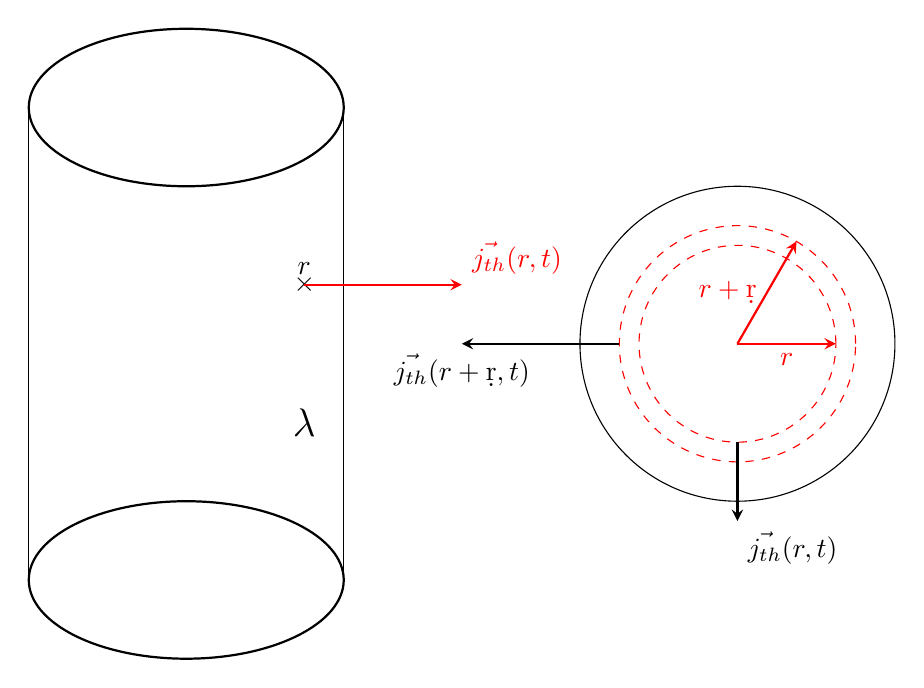
\begin{tikzpicture}[scale=1]  
                    % \helpgrid{3}{3}
                    \draw (-2,-3)--++(0,6);
                    \draw (2,-3)--++(0,6);
                    \draw [thick] (0,-3) ellipse (2cm and 1cm);
                    \draw [thick] (0,3) ellipse (2cm and 1cm);
                    \node at (1.5,-1) {\Large$\lambda$};
                    \coordinate (R) at (1.5,0.75);
                    \node at (R) {$\times$};
                    \node at (R) [above] {$r$};
                    \draw[red,->,-stealth,text=red,thick] (R)--++(2,0) node [above right] {$\vec{j_{\text{th}}}(r,t)$};

                    \coordinate (O) at (7,0);
                    \draw [color=black,smooth] (O) circle (2);
                    \draw [color=black,smooth,red,dashed] (O) circle (1.25);
                    \draw [color=black,smooth,red,dashed] (O) circle (1.5);
                    \draw[red,->,-stealth,text=red,thick] (O)--++(1.25,0) node [below, midway] {$r$};
                    \draw[red,->,-stealth,text=red,thick] (O)--++(0.75,1.3) node [left,midway] {$r+\d r$};

                    \draw[->,-stealth,thick] (7,-1.25)--++(0,-1) node [below right] {$\vec{j_{\text{th}}}(r,t)$};
                    \draw[->,-stealth,thick] (5.5,0)--++(-2,0) node [below] {$\vec{j_{\text{th}}}(r+\d r,t)$};
                \end{tikzpicture}
                \caption{Équation locale de la conservation de l'énergie en géométrie cylindrique.}    
                \label{fig:equation_locale_conservation_energie_1d_cylindrique}
            \end{figure}

            On a, via un développement limité de $rj_{\text{th}}(r,t)$,
            \begin{equation}
                \delta P_{\text{th}}^{\text{ext}}=j_{\text{th}}(r,t)\times 2\pi rL-j_{\text{th}}(r+\d r,t)\times 2\pi(r+\d r)L=-2\pi L\d r\frac{\partial}{\partial r}\left(rj_{\text{th}}(r,t)\right).
            \end{equation}

            Le premier principe s'écrit
            \begin{equation}
                \frac{\d}{\d t}(\delta U)=\delta P_{\text{th}}^{\text{ext}}=-2\pi L\d r\frac{\partial}{\partial r}\left(rj_{\text{th}}(r,t)\right)=u_{\text{vol}}(r,t)\times2\pi r\d rL.
            \end{equation}
            Ainsi, on a 
            \begin{equation}
                \boxed{
                    \frac{\partial u_{\text{vol}}(r,t)}{\partial t}+\frac{1}{r}\frac{\partial}{\partial r}\left(rj_{\text{th}}(r,t)\right)=0.
                }
            \end{equation}
            En phase condensée, on a $\dfrac{\partial u_{\text{vol}}(r,t)}{\partial t}=\mu c\dfrac{\partial T}{\partial t}$, où [c]=\si{\joule\per\kilogram\per\kelvin}.

        \subsubsection{Géométrie sphérique}

            On fait l'hypothèse que la température $T(r,t)$ dépend juste du rayon $r$ et du temps $t$, et que $\vec{j_{\text{th}}}=j_{\text{th}}(r,t)\vec{u_r}$, voir la Figure~\ref{fig:equation_locale_conservation_energie_1d_spherique}. On considère l'espace entre deux sphères de rayon $r$ et $r+\d r$.
        
            \begin{figure}
                \centering
                \tikzsetnextfilename{equation_locale_conservation_energie_1d_spherique}
                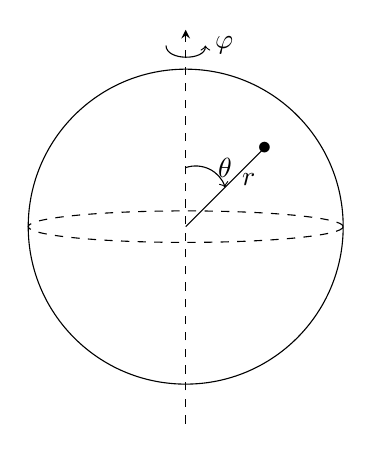
\begin{tikzpicture}[scale=1]  
                    % \helpgrid{3}{3}
                    \coordinate (O) at (0,0);
                    \draw [color=black,smooth] (O) circle (2);
                    \draw [dashed, ->, -stealth] (0,-2.5)--(0,2.5);
                    \draw (O)--++(1,1) node [below, pos=0.8] {$r$};
                    \node at (1,1) {$\bullet$};
                    \draw [->] (0,0.75) to [bend left=45] (0.5,0.5) node [above] {$\theta$};
                    \draw [->] (-0.25,2.3) to [bend right=90] (0.25,2.3) node [right] {$\varphi$};
                    \draw [color=black,smooth,dashed] (O) ellipse (2 and 0.2);
                \end{tikzpicture}
                \caption{Équation locale de la conservation de l'énergie en géométrie sphérique.}    
                \label{fig:equation_locale_conservation_energie_1d_spherique}
            \end{figure}

            En effectuant un développement deTaylor de $r^{2}j_{\text{th}}(r,t)$, on a 
            \begin{align}
                \delta P_{\text{th}}^{\text{ext}}
                &=
                j_{\text{th}}(r,t)\times 4\pi r^{2}-j_{\text{th}}(r+\d r,t)\times4\pi(r+\d r)^{2},\\
                &=-4\pi\d r\frac{\partial}{\partial r}\left(r^{2}j_{\text{th}}(r,t)\right).
            \end{align}

            Le premier principe s'écrit
            \begin{equation}
                \frac{\d(\delta U)}{\d t}=\delta P_{\text{th}}^{\text{ext}}=4\pi r^{2}\d r\frac{\partial u_{\text{vol}}}{\partial t},
            \end{equation}
            d'où
            \begin{equation}
                \boxed{
                    \frac{\partial u_{\text{vol}}}{\partial t}+\frac{1}{r^{2}}\frac{\partial}{\partial r}\left(r^{2}j_{\text{th}}(r,t)\right)=0.
                }
            \end{equation}

        \subsubsection{Généralisation en 3D dans une géométrie quelconque}
            
            Dans un volume $\mathcal{V}$ quelconque, on écrit
            \begin{equation}
                \begin{aligned}
                    U(t)&=\iiint_{\mathcal{V}}u_{\text{vol}}(\vec{r},t)\d\tau,\\
                    U(t+\d t)&=\iiint_{\mathcal{V}}u_{\text{vol}}(\vec{r},t+\d t)\d\tau,\\
                \end{aligned}
            \end{equation}
            où $\d\tau$ est un volume infinitésimal. Alors
            \begin{equation}
                \d U=U(t+\d t)-U(t)=\iiint_{\mathcal{V}}\frac{\partial u_{\text{vol}}}{\partial t}(\vec{r},t)\d t\d\tau.
            \end{equation}
            On fait l'hypothèse que l'on peut \og sortir\fg~le terme $\d t$ de l'intégrale. On écrit
            \begin{equation}
                P_{\text{th}}^{\text{ext}}=-\oiint_{S}\vec{j}_{\text{th}}\cdot\vec{n}^{\text{ext}}\d S,
            \end{equation}
            car il y a une perte si $\vec{j}_{\text{th}}\cdot\vec{n}^{\text{ext}}>0$. Le premier principe s'écrit 
            \begin{equation}
                \frac{\d U}{\d t}=P_{\text{th}}^{\text{ext}},
            \end{equation}
            et en utilisant le théorème d'Ostrogradski,
            \begin{equation}
                \iiint_{\mathcal{V}}\frac{\partial u_{\text{vol}}(\vec{r},t)}{\partial t}\d\tau=-\oiint_{S}\vec{j}_{\text{th}}\cdot\vec{n}^{\text{ext}}\d S=-\iiint_{\mathcal{V}}\mathrm{div}~\vec{j}_{\text{th}}(\vec{r},t)\d\tau.
            \end{equation}
            Ainsi, on a 
            \begin{equation}
                \boxed{
                    \frac{\partial u_{\text{vol}}}{\partial t}+\mathrm{div}~\vec{j}_{\text{th}}=0.
                }
            \end{equation}

        \subsubsection{Généralisation avec terme source}

            En plus de la conduction thermique, on a un apport énergétique en volume.

            \begin{example}
                L'effet Joule ajoute une puissance dû au travail électrique
                \begin{equation}
                    P_{\text{vol}}=\vec{j}\cdot\vec{E}=\sigma E^{2}=\frac{j^{2}}{\sigma}>0.
                \end{equation}
            \end{example}
            \begin{example}
                L'énergie dégagée par une réaction chimique exothermique rajoute une puissance
                \begin{equation}
                    P_{\text{vol}}=\frac{1}{\mathcal{V}}\Delta_r H^{0}\frac{\partial\xi}{\partial t}.
                \end{equation}
            \end{example}

            On adapte donc le bilan précédent en écrivant
            \begin{equation}
                \frac{\d U}{\d t}=P_{\text{th}}^{\text{ext}}+\iiint_{\mathcal{V}}P_{\text{vol}}(\vec{r},t)\d\tau,
            \end{equation}
            d'où
            \begin{equation}
                \boxed{
                    \frac{\partial u_{\text{vol}}}{\partial t}+\mathrm{div}~\vec{j}_{\text{th}}=P_{\text{vol}}.
                }
            \end{equation}

            \begin{example}
                Dans le cas de l'effet Joule, on a 
                \begin{equation}
                    \mu c\frac{\partial T}{\partial t}+\mathrm{div}~\vec{j}_{\text{th}}=P_{\text{vol}}=\vec{j}\cdot\vec{E}>0.
                \end{equation}
                Or 
                \begin{equation}
                    \frac{\partial}{\partial t}\left(\frac{\varepsilon_{0}E^{2}}{2}+\frac{B^{2}}{2\mu_0}\right)+\mathrm{div}~\vec{\Pi}=-\vec{j}\cdot\vec{E}<0.
                \end{equation}
                Cela caractérise le changement de point de vue champ/conducteur.
            \end{example}

    \subsection{Équation de la chaleur/diffusion thermique}
            
        On fait l'hypothèse qu'il n'y a que de la conduction pure. L'idée est que l'on a deux ingrédients : la loi de Fourier, et l'équation locale de la conservation de l'énergie. On peut donc combiner les choses pour obtenir l'équation de la chaleur.

        \subsubsection{Cas 1D en géométrie cartésienne}
            
            On a 
            \begin{equation}
                \vec{j}_{\text{th}}(x,t)=-\lambda\vec{\mathrm{grad}}~T=-\lambda\frac{\partial T}{\partial t}(x,t)\vec{u_x},
            \end{equation}
            et
            \begin{equation}
                \mu c\frac{\partial T}{\partial t}+\frac{\partial j_{\text{th}}}{\partial x}=0.
            \end{equation}
            Ainsi, en posant
            \begin{equation}
                \boxed{
                    D=\frac{\lambda}{\mu c},
                }
            \end{equation}
            le coefficient de diffusion thermique, on a 
            \begin{equation}
                \boxed{
                    \frac{\partial T}{\partial t}=D\frac{\partial^{2}T}{\partial x^{2}}.
                }
            \end{equation}
            L'unité de $D$ est le \si[]{\metre\square\per\second}.

        \subsubsection{Géométrie cylindrique}
            
            On écrit 
            \begin{equation}
                \begin{aligned}
                    \vec{j}_{\text{th}}(x,t)&=-\lambda\frac{\partial T}{\partial r}\vec{u_r},\\
                    \mu c\frac{\partial T}{\partial t}+\frac{1}{r}\frac{\partial}{\partial r}\left(rj_{\text{th}}(\vec{r},t)\right)&=0,
                \end{aligned}
            \end{equation}
            d'où
            \begin{equation}
                \boxed{
                    \frac{\partial T}{\partial t}=D\frac{1}{r}\frac{\partial}{\partial t}\left(r\frac{\partial T}{\partial t}\right).
                }
            \end{equation}

        \subsubsection{Géométrie sphérique}
            
            On écrit 
            \begin{equation}
                \begin{aligned}
                    \vec{j}_{\text{th}}(x,t)&=-\lambda\frac{\partial T}{\partial r}\vec{u_r},\\
                    \mu c\frac{\partial T}{\partial t}+\frac{1}{r^{2}}\frac{\partial}{\partial r}\left(r^{2}j_{\text{th}}(\vec{r},t)\right)&=0,
                \end{aligned}
            \end{equation}
            d'où
            \begin{equation}
                \boxed{
                    \frac{\partial T}{\partial t}=D\frac{1}{r^{2}}\frac{\partial}{\partial t}\left(r^{2}\frac{\partial T}{\partial t}\right).
                }
            \end{equation}
        
        \subsubsection{Géométrie quelconque}
            
            On écrit
            \begin{equation}
                \begin{aligned}
                    \vec{j}_{\text{th}}=-\lambda\vec{\mathrm{div}}~T,\\
                    \mu c\frac{\partial T}{\partial t}+\mathrm{div}~\vec{j}_{\text{th}}&=0,
                \end{aligned}
            \end{equation}
            d'où
            \begin{equation}
                \boxed{
                    \frac{\partial T}{\partial t}=D\Delta T.
                }
            \end{equation}

        \subsubsection{Avec terme source}

            C'est la même chose sauf que l'on a 
            \begin{equation}
                \mu c\frac{\partial T}{\partial t}+\mathrm{div}~\vec{j}_{\text{th}}=P_{\text{vol}},
            \end{equation}
            d'où
            \begin{equation}
                \boxed{
                    \frac{\partial T}{\partial t}=D\Delta T+\frac{P_{\text{vol}}}{\mu c}.
                }
            \end{equation}

    \subsection{Création d'entropie par diffusion}
            
        On se place dans le cas unidimensionnel et que l'on est en régime stationnaire. On a donc $T(x)$ et $\vec{j}_{\text{th}}=-\lambda\frac{\partial T}{\partial x}\vec{u_x}$. On fait l'hypothèse que l'on a $\frac{\d T}{\d x}<0$. On reprend la Figure~\ref{fig:equation_locale_conservation_energie_1d_cartesien} et on applique le second principe à $[x,x+\d x]$, on a 
        \begin{equation}
            \d(\delta S)=\delta S_e+\delta S_c,
        \end{equation}
        pendant $\d t$. Comme on est en régime stationnaire, on a $\d(\delta S)=0$. Ainsi, $\delta S_c=-\delta S_c$. Or, en notant $A$ la section verticale, on a
        \begin{equation}
            \delta S_e=\frac{j_{\text{th}}(x) A\d t}{T(x)}+\frac{-j_{\text{th}}(x+\d x)A\d t}{T(x+\d x)}.
        \end{equation}
        On est en régime permanent, on a donc
        \begin{equation}
            \frac{\partial u_{\text{vol}}}{\partial t}=0=-\mathrm{div}~\vec{j}_{\text{th}}=-\frac{\partial j_{\text{th}}}{\partial x}=0.
        \end{equation}
        Donc 
        \begin{equation}
            j_{\text{th}}(x)=\mathrm{constante}=-\lambda\frac{\d T}{\d x}=-\lambda\frac{T_2-T_1}{L}.
        \end{equation}
        On a alors
        \begin{equation}
            \delta S_e
            =j_{\text{th}}A\d t\left[
                \frac{1}{T(x)}-\frac{1}{T(x+\d x)}
            \right]=A\d t\left(-\lambda\frac{\d T}{\d x}\right)\d x\frac{\frac{\d T}{\d x}}{T(x)^{2}},
        \end{equation}
        donc $\delta S_e=-\delta S_c<0$, et ce peu importe le signe de $\frac{\d T}{\d x}$. Ainsi, $\delta S_c>0$ : \textbf{c'est le caractère fondamentalement irréversible des phénomènes de diffusion}.